
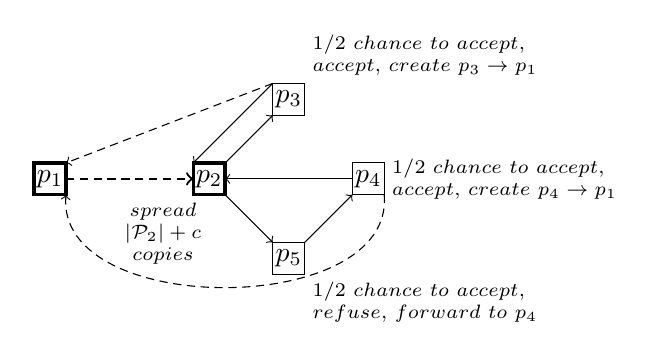
\begin{tikzpicture}[scale=1.15]
  
  \draw[fill=white, very thick] (0pt, 0pt)
  node{$p_1$} +(-5pt,-5pt) rectangle +(5pt,5pt);

  \begin{scope}[shift={(75pt,0pt)}]
  \draw[fill=white, very thick]
  (-25pt, 0pt) node{$p_2$} +(-5pt,-5pt) rectangle +(5pt,5pt);
  \draw[fill=white] (0pt,  25pt) node{$p_3$} +(-5pt,-5pt) rectangle +(5pt,5pt);
  \draw[fill=white] ( 25pt, 0pt) node{$p_4$} +(-5pt,-5pt) rectangle +(5pt,5pt);
  \draw[fill=white] (0pt, -25pt) node{$p_5$} +(-5pt,-5pt) rectangle +(5pt,5pt);


  \draw[->] (-20pt, 5pt) -- (-5pt, 20pt); 
  \draw[->] (-20pt,-5pt) -- (-5pt,-20pt); 
  \draw[->] ( 5pt,-20pt) -- (20pt, -5pt); 
  \draw[->] (20pt,  0pt) -- (-20pt, 0pt); 
  \draw[->] (-5pt, 30pt) -- (-30pt, 5pt); 

  \draw[->, thick, densely dashed] (-70pt, 0pt) -- (-30pt, 0pt); 
  \draw[->, densely dashed] (-5pt, 30pt) -- (-70pt, 5pt); 
  \draw[->, densely dashed] (30pt, -5pt)to[out=-85,in=-95](-70pt,-5pt);

  \scriptsize
  \draw (-25pt,-5pt) node[align=center,anchor=north east]
  {$spread$\\$|\mathcal{P}_2|+c$\\$copies$};
  \draw (5pt,-30pt) node[align=left,anchor=north west]
  {$1/2$ $chance$ $to$ $accept,$\\$refuse,$ $forward$ $to$ $p_4$};
  \draw (5pt, 30pt) node[align=left,anchor=south west]
  {$1/2$ $chance$ $to$ $accept,$\\$accept,$ $create$ $p_3 \rightarrow p_1$};
  \draw (30pt, 0pt) node[align=left,anchor=west]
  {$1/2$ $chance$ $to$ $accept,$\\$accept,$ $create$ $p_4 \rightarrow p_1$};
  \end{scope}
  
%%  \small
%%  \begin{scope}[shift={(130pt,0pt)}]
%%    \draw[fill=white](5pt, 0pt)node{$p_x$}+(-5pt,-5pt) rectangle +(5pt,5pt);
%%    \draw (10pt,0pt) node[anchor=west]{Peer $p_x$};
%%    \draw[->](0pt, -12pt)--(10pt, -12pt) node[anchor=west]{Established link};
%%    \draw[->, densely dashed](0pt, -19pt)--(10pt, -19pt)
%%    node[anchor=west]{New link};
%%    
%%  \end{scope}
  
\end{tikzpicture}